% Copyright 2022 David W. Hogg (NYU) and Andy Casey (Monash)

% To-Do items
% -----------
% - Audit for rigid terminology. HOGG is currently liking ``combined spectrum'' for the model expectation, for example. And "standard practice" for the traditions of our field.
% - Audit and fix the sign applied to $\Delta x_i$ everywhere. Wrong relative to code?
% - Write about the two input-data cases.
% - See bug list in code for other issues with the text--code relationship (noise model; line-formation model).
% - Audit for its / it's. Hogg has issues with this.
% - Deal with all HOGG, ANDY, ARC, XXX, YYY, CITE, etc.

\documentclass[modern]{aastex631}
\usepackage[utf8]{inputenc}
\usepackage{amsmath}

% page and document setup
\renewcommand{\twocolumngrid}{}
\addtolength{\topmargin}{-0.35in}
\addtolength{\textheight}{0.6in}
\setlength{\parindent}{3.5ex}
\renewcommand{\paragraph}[1]{\medskip\par\noindent\textbf{#1}~---}

% figure setup
\usepackage{graphicx}
\usepackage{xcolor}
\usepackage[framemethod=tikz]{mdframed}
\usetikzlibrary{shadows}
\definecolor{captiongray}{HTML}{555555}
\mdfsetup{%
  innertopmargin=2ex,
  innerbottommargin=1.8ex,
  linecolor=captiongray,
  linewidth=0.5pt,
  roundcorner=1pt,
  shadow=false,
}
\newlength{\figurewidth}
\setlength{\figurewidth}{0.75\textwidth}

% text macros
\shorttitle{don't interpolate your data}
\shortauthors{hogg \& casey}
\newcommand{\documentname}{\textsl{Article}}
\newcommand{\sectionname}{Section}

% math macros
\newcommand{\unit}[1]{\mathrm{#1}}
\newcommand{\mps}{\unit{m\,s^{-1}}}
\newcommand{\kmps}{\unit{km\,s^{-1}}}

% notes

\sloppy\sloppypar\raggedbottom\frenchspacing
\begin{document}

\title{\Huge Don't interpolate the data!}
% ARC: I changed this to "Don't interpolate the data!"? because you can't like, own data, man.
% (but you can change it back if you prefer)

\author[0000-0003-2866-9403]{David W. Hogg}
\affiliation{Center for Cosmology and Particle Physics, Department of Physics, New York University}
\affiliation{Max-Planck-Institut f\"ur Astronomie, Heidelberg}
\affiliation{Flatiron Institute, a division of the Simons Foundation}

\author[0000-0003-0174-0564]{Andrew R. Casey}
\affiliation{School of Physics \& Astronomy, Monash University}
\affiliation{Centre of Excellence for Astrophysics in Three Dimensions (ASTRO-3D)}

\begin{abstract}\noindent
When there are many observations of an astronomical source---many images with different dithers, or many spectra taken at different barycentric velocities---it is often tempting to shift and stack the data, to (for example) make a high signal-to-noise average image or mean spectrum.
Bound-saturating measurements are made not by manipulating data, but instead by manipulating a likelihood function, where the data are treated as fixed, and model parameters are modified to fit the data.
Traditional shifting and stacking of data can be converted into a model-fitting procedure, such that no data are ever harmed, and yet the output is the shift-adjusted mean.
The key component of this conversion is a spectral model that is completely flexible but also a continuous function of wavelength (or position in the case of imaging) that can represent any signal being measured by the device after any reasonable translation (or rotation or field distortion).
The benefits of a modeling approach are myriad:
The sacred data never are modified.
Noise maps, data gaps, and bad-data masks don't require interpolation.
The output can take the form of a spectrum evaluated on a pixel grid, as is traditional.
The noise in the output spectrum becomes uncorrelated across neighboring pixels. 
The only cost is a small increase in computational complexity.
We demonstrate all of these things with a small data example and we provide open-source sample code for re-use.
\end{abstract}

\keywords{Foo --- Bar --- HOGG}

\section*{}\clearpage
\section{Introduction}\label{sec:intro}

It would be wrong to say that the practice of astronomy is, basically, \emph{staring at the sky}.
That said, staring at the sky is a big part of what we do.
And the way we do it, usually, is this:
We take many individual images of our target with exposure times that are long enough to make read noise irrelevant (if possible) while at the same time short enough to avoid saturation (of what we care about).
We then shift and average (maybe median?) those images to get the highest possible signal-to-noise on our target.
This, fundamentally, is the technology underlying the \textsl{Hubble Deep Field} (\citealt{hdf}),
the \textsl{APOGEE} spectroscopic survey (\citealt{apogee}),
and the future Rubin Observatory \textsl{LSST} (\citealt{lsst}), among countless other projects.

Is it astronomical blasphemy to say that this practice is \emph{wrong?}
It is wrong because minimum-variance unbiased estimators require care in their construction; they are (often) maximum-likelihood estimators (\citealt{something}). % HOGG
The deep, high signal-to-noise image or spectrum we seek is a statistical estimate of the image or spectrum, given the noisy data of the individual exposures.
Noisy data are combined to make a measurement by building and optimizing a likelihood, not by shifting and stacking the input data.
Of course we don't always think of an image or a spectrum of the sky as the result of applying an \emph{estimator}, but it is.
It is just a simultaneous estimate of a lot of different components (a lot of different pixels; all the pixels in the combined image or spectrum).

We are in a period in astrophysics in which exceedingly precise measurements are expected, in both imaging and spectroscopy projects.
In spectroscopy, in particular, high signal-to-noise spectral measurements are expected to obtain surface-abundance measurements with precisions a few percent, and radial-velocity measurements with precisions of up to one ten-thousandth of a \emph{pixel} (in terms of the Doppler shift).
Spectral combination methods that distort absorption (or emission) lines will translate into biases, errors, or increased variance in these measurements.
Spectral combination methods that correlate the noise in the outputs will translate into increased variance, and necessitate more sophisticated downstream measurement techniques (which don't really exist at present).

One of the great things about the standard practice---the simple process of shifting and stacking the data---is that this procedure makes almost no assumptions about what the output, combined image or spectrum will look like.
It isn't really a ``model'' for the data; it is more like a ``summary'' of the data.
When we switch to a statistical-inference framework, we have to choose some form or basis for expressing the combined image.
In what follows we use a maximally parameterized model, in the sense that we choose an expression for the functions or function space that has as many parameters as the output image has pixels.
That means that the approach we take does not get its power from the choice of parameterized functions for the output:
Indeed it has just as much freedom as the shifting-and-stacking standard practice.
The forward-modeling we recommend gets its power from the fact that it generates the data directly and without manipulation.

The data are never manipulated when using an estimator (in contrast to standard practice), but (for us) the functional requirements are the same as with standard practice:
We consider here only procedures that start with the individual, single-epoch observations as inputs, along with noise estimates, bad-pixel masks, and perhaps bit-flags; and we consider only procedures that end with an output ``combined image'' or ``combined spectrum'' that is a set of intensity of flux values on a pixel grid, along with uncertainty estimates and metadata flags.
That is, the only difference between standard practice and the forward model that we advocate is the purely in the nature of the estimator.
Unlike the shift-and-coadd approach, the estimator we will deliver will be insensitive to under- or poorly-sampled data, which is not uncommon when astronomical seeing accidentally gets excellent, or in spectrographs that have limited detector pixels (for example, \citealt{apogeehardware}).
As we will show, an estimator also often yields a more faithful estimate of the \emph{true} spectrum, and almost always better noise properties.
Both of these results make our results better for any subsequent precision measurements (e.g., radial velocities, chemical abundances).
But importantly, we aren't proposing a change to the \emph{format} of the input or outputs of spectral or image combination.

% Hogg's email epiphany:
% 1. I think I figured out what Blanton means by saying that interpolation of the data is a kind of fitting. It is! But those fits can’t be combined well because the fits are infinitely over-parameterized. If the interpolation was done approximately with a finite-parameter fit, we could interpolate and then average just fine. I’m writing this here to remind myself of this epiphany for when I come back online and write a subsection about this in the paper.

% Hogg: what do you want to do about this?

The approach we propose differs from interpolation in a subtle way. 
Interpolation could be described as computing new values at arbitrary positions based on an exising set of known data points. 
Instead, here we propose to construct a continuous spectral model for the data, where we then evaluate that model on the given set of output positions (pixels).
The \emph{output product} is the same form as what one would expect from an interpolation procedure (e.g., computed values along some array of positions), but the \emph{procedure} differs from interpolation. When interpolating data the basis functions are explicitly constructed from the data, whereas here we construct a forward model that is maximally consistent with the data, and evaluated at new positions.

The ideas here aren't novel; many projects have avoided data interpolation previously.
For one example, the \textsl{COMBO-17} survey (\citealt{combo17}) took many images of the sky in many bands, and did not co-add the data prior to making measurements, in part to avoid mixing different point-spread functions and pixel samplings.
For another, what we propose below is actually a sub-problem of the problem solved by the \textsl{wobble} method for determining stellar radial velocities (\citealt{wobble}); \textsl{wobble} is more general because it also includes a tellurics model and also tellurics and stellar variability models.
Plus it learns (it isn't told) the epoch-to-epoch spectral shifts.
There is a heritage for what's presented here in the ``optimal extraction'' literature (for example, \citealt{oe}, \citealt{froe}, \citealt{sp}):
Optimal extraction describes a process of extracting a one-dimensional spectral signal from a two-dimensional spectrograph image when that extraction proceeds by forward modeling the two-dimensional data.
One amusing point, which is out of scope here, is that if the data that are being combined are extracted one-dimensional spectra, and those are, in turn, optimal extractions, then there is a better method that moves this spectral combination method directly into the two-dimensional data.
We hope for a future in which one-dimensional spectra are never extracted from two-dimensional images; in this future the two-dimensional data are the sacred data, not the extractions.

In real applications, the spectra we extract are often of variable sources, or taken at different position angles on extended objects, such that we don't expect each epoch to be identical.
Similarly, the \textsl{LSST} data are being taken the way they because the sky (and point-spread function) will vary.
That means that we are only considering here the very easiest case.
However, we note that all standard shift-and-coadd methods make these non-variable assumptions implicitly.
Part of our contribution in this \documentname{} is to make implicit assumptions explicit, in \sectionname~\ref{sec:assumptions}.

HOGG: Most important: Say here why you should never want to do this at all! % ARC: I think you've covered this by talking about the two-dimensional data.
Comment on a spectrum being too low in s/n to measure a Na line...!! % ARC: I don't remember what the context is for this

\section{Concepts and assumptions}\label{sec:assumptions}

What we do here can apply to almost any astronomical signals, but we are going to specialize to multi-epoch astronomical spectra for specificity.
We are going to make many other assumptions too, all of which are discussed in this \sectionname.

\paragraph{Multi-epoch spectra with shifts}
We will assume that there are $n$ observations (epochs) of the same star (or maybe of different stars or quasars, say, that are assumed to be more-or-less identical, intrinsically, but let's think of a single star for now).
Each of these observations $i$ (with $1\leq i\leq n$) produces a one-dimensional observed (noisy) image $y_i$.
The $y_i$ can be thought of as $m_i$-vectors in what follows, where $m_i$ is the number of pixels in the $i$-th spectrum.
The different observations are made at different relative velocities (star minus spectrograph) such that the images are shifted by a different shift $\Delta x_i$ relative to the detector or extracted wavelength grid.

\paragraph{Shift operators}
Because the shifts might be non-linear, the shifts $\Delta x_i$ won't be pure numbers but something more like shift operators.
That is, if there were a true spectrum $\tilde{y}$, each individual noisy image $y_i$ would be related to that true spectrum by a shift operator acting on that true spectrum, plus noise.
We will assume here that (from some external information) we know these shift operators very accurately.
This is often not true, of course; we will return to this point in the discussion.

\paragraph{Wavelength calibration}
We will assume that, for every $m_i$-pixel image $y_i$ we also have a $m_i$-vector (or list) $x_i$ of pixel positions, such that each element of $x_i$ gives an accurate and precise value for the wavelength (or position in the spectrograph, in some settings) for each pixel of the image $y_i$.
That is, the device is well calibrated, and we know all the housekeeping data we need for image $y_i$.

\paragraph{Noise model}
Each observation is noisy.
We will assume that the noise has known properties, and especially that it is additive, (nearly) zero-mean and (nearly) Gaussian in form, with known variance.
Under these assumptions, each spectrum $y_i$ has an associated variance tensor $C_i$.
If $y_i$ is an $m_i$-vector, then $C_i$ is a nonnegative-definite $m_i\times m_i$ 2-tensor.
We don't need to assume that the different pixels of the spectrum received independent noise, but we do assume that each epoch $i$ has an independent noise draw.

\paragraph{Bad-pixel masks}
Occasionally (or frequently) some of the pixels of a spectrum $y_i$ might be bad---affected by cosmic rays or electronics issues---such that there is a bad-pixel mask $b_i$ associated with each spectrum $y_i$.
This mask has value 1 in the locations in all good pixels, and 0 in the locations of all bad pixels.

\paragraph{Bit-flags}
A bit-flag is often used to store meta data about a pixel that otherwise cannot be encoded by the spectrum $y_i$ or its asssociated variance tensor $C_i$ (e.g., poorly described line spread function). 
We often want to propagate this meta data to appropriate pixels in the combined spectrum. 
These bit-flag masks are usually encoded as integers with up to $F$ potential flags, allowing for all (or a subset of) flags to be encoded as a single value $\sum^{F}_{f=0} 2^f$. 
This bit-flag mask can be separated into $F$ masks where each has value 1 in the locations where the flag is marked, and 0 in the locations where it is not.

\paragraph{Data gaps}
There is no assumption here that all the $y_i$ have the same number of pixels $m_i$, nor that the pixel grid is in any sense uniform or complete.
That is, there can be gaps and spaces in the wavelength coverage of the spectra, as there are at chip gaps and where the detector has bad columns.

\paragraph{Pixel-convolved line-spread function}
The spectrograph has something like a point-spread function or line-spread function, which, in the case of spectrosccopy, sets the shape of an unresolved spectral line.
In general it depends on the slit or fiber width, the spectrograph resolution and optics, instrument focus, and the properties of the detector.
In what follows we will not build a model of any of this.
Instead we will assume that there is a relatively constant pixel-convolved line-spread function (PCLSF), constant both in time, and constant with respect to the shifts $\Delta x_i$ we see in our data set.
We consider only the PCLSF, because then the sampling by the detector pixels does not require any additional convolution.
That is, when the PCLSF is used to model a spectrum, the projection onto the pixels is just a sampling of the function at the pixel centers, and does not involve any convolution over the face of the pixel.
All that said, we won't explicitly model or use the PCLSF in what follows; we will just assume that our continuous spectral model is a model for the pixel-convolved, finite-resolution spectrum; we won't be doing any convolutions in comparing models and data.

In many cases the LSF or PSF is actually substantially different in different exposures.
This leads to spectral (or image) variations, and violate the assumptions of this model (and also the implicit assumptions underlying standard practice).
We won't address this kind of variability here, except in some discussion at the end.

\paragraph{Continuous spectral model} 
In what follows we are going to avoid interpolating the \emph{data} by having a spectral \emph{model} that can be arbitrarily and losslessly interpolated.
That means that the spectral model must be a representation of a continuous one-dimensional function.
If we were working on two-dimensional images, the model would have to be a representation of a continous two-dimensional function.

\paragraph{Linear basis or mixture models}
The simplest kind of model for a continuous function is a sum or mixture or linear combination of continuous basis functions.
These could be sines and cosines for a Fourier series model.
They could be spline (or sinc or Lanczos) cardinal basis functions.
They could be wavelets.
The point is that if we use a linear basis, and assume that noises are Gaussian, we will get closed-form expressions for the data combination.
Thus we will use a linear basis.

\paragraph{Band limit}
We say that a signal is \emph{band-limited} if it has no frequency content above some highest possible cutoff frequency.
There is a weird sense in which data from a spectrograph both is, and is not, band limited.
It is band limited in that the spectrograph is finite in resolution, such that no real spectroscopic signal can show features narrower than the PCLSF.
It is not band-limited in that the photon noise in the device is independent (or close to independent) from pixel to pixel, such that the noise contribution to each observation $y_i$ has support at all spatial frequencies.

One interesting question in what follows is whether the forward model we build for the data should itself be restricted to the band limit defined by the spectrograph resolution, or whether it should permit higher frequencies.
It might surprise the reader to learn that we prefer to let the model capture higher frequencies, even when we think they shouldn't be there for any reasons other than noise, given the hardware.
More on this below.

\paragraph{Critical sampling}
Because of considerations related to the Nyquist frequency on a uniform grid, it is valuable for a spectrograph to have a pixel spacing on the device that is smaller than the width of the PCLSF.
Specifically, it is valuable for there to be two or three pixels across the full-width at half-maximum (FWHM) of the PCLSF.
This keeps the band-limited part of the spectroscopic signal well-sampled in the data.
There are spectrograph that don't have pixel scales this fine (for example, \textsl{APOGEE}; \citealt{apogee}); in these cases what we are proposing here is \emph{even more important} than it is in the well-sampled case.
This will become obvious in the experiments below.

\paragraph{Non-uniform fast Fourier transform}
In the special case that the spectral model is a Fourier series, there are very useful and fast tools for interpolation, including especially the non-uniform fast Fourier transform (for example, \citealt{finufft}).

\paragraph{Time variability}
When we average data (or build a static model of multi-epoch data), we are implicitly assuming that there is no intrinsic variability to the source being observed.
That is, we are assuming that the changes from observation to observation are solely from either the shifts $\Delta x_i$ or from the noise.
We interpolate the model to account for the shifts, and we combine data to beat down the noise.
There are situations in which there is substantial time variability and these approaches are still valid, and there are modified approaches.
We will discuss these changes and generalizations at the end.

\paragraph{Bias, sky, tellurics, flat-field, normalization}
In what follows, we will assume that the input data are well calibrated in various ways.
In particular, we will assume that the images or spectra have been bias-corrected, sky-subtracted, flat-fielded, and tellurics-corrected sufficiently well that the different observations $y_i$ can be seen as observations of the same underlying or intrinsic signal.
Alternatively, the input data might be continuum-normalized or pseudo-continuum-normalized.
Again, the assumption is that the different calibrated or processed observations are of the same underlying signal.
If there are multiple signals participating, the model would have to expand into something like \textsl{wobble} (\citealt{wobble}).

\section{Method}\label{sec:method}

The problem set-up is that there are $N$ spectral measurements $y_i$ (with $1\leq i\leq N$), each of which is a $M_i$-pixel list of intensities (fluxes maybe).
Different observations $i$ might have different numbers $M_i$ of pixels.
The $M_i$ pixels are associated with an $M_i$-length list of positions (wavelengths or log-wavelengths) $x_i$.
Each measurement or observation $i$ is shifted by a shift operator $\Delta x_i$, which can be thought of as a length-$M_i$ list of pixel offsets or shifts, such that the ``rest frame'' or ``unshifted'' positions corresponding to the length-$M_i$ list of data $y_i$ is the list of differences $x_i - \Delta x_i$.
The goal is to get a combined spectrum that represents the mean of these spectra, in the common rest frame.

The spectral expectation model $f(x;\theta)$, which will be a representation for our combined spectrum, is a function of $x$ controlled by a list $\theta$ of $P$ linear parameters $a_j$ (with $1\leq j\leq P$).
This function will be very flexible; possibly even an interpolation of control points or a Fourier series; the number $P$ will be roughly the number of pixels we want in our output combined spectrum.
The statistical model underlying can be expressed qualitatively as
\begin{align}
    y_i &= f(x_i + \Delta x_i;\theta) + \mbox{noise} \\
    f(x;\theta) &= \sum_{j=1}^P a_j\,g_j(x) ~,
\end{align}
where we are being a bit loose with terminology (since $x_i$ is a set of positions, not just one position), the noise is additive (but not yet specified), and each of the $P$ functions $g_j(x)$ is a basis function of the representation.

The noise model is additive (as noted above) and we will assume that the noise contributing to observation $y_i$ is zero-mean and Gaussian, with a known $M_i\times M_i$ variance tensor $C_i$ (or its inverse $C_i^{-1}$).
If the raw pixel measurements are independent, which they often are (and are often assumed to be), then the $C_i$ (or $C_i^{-1}$) matrices will be diagonal matrices with the individual pixel variances (or inverse variances) down the diagonals.
In many cases you don't know (or aren't provided with) the individual pixel variances, and you are just co-adding data with uniform weights.
That choice, for our purposes, is equivalent to setting every inverse variance matrix $C_i^{-1}$ to the $M_i\times M_i$ identity matrix.
That's permitted!
It is no worse a choice than it was (in the past) when you averaged your input data without thinking about noise variances or weights.
Another sensible default choice would be to set each inverse matrix $C_i^{-1}$ to the identity times the exposure time, such that the eventual math we do will weight the data by the exposure times.
That is, you do not need to know the noise variances accurately (or even at all) to execute the forthcoming procedure; but if you do know them, it is good to use them.

If you additionally have a bad-pixel mask $b_i$ associated with each observation $y_i$, the bad-pixel mask can be used simply to zero out the corresponding bad rows and columns of the inverse covariance matrix $C_i^{-1}$.
Importantly, the bad data get zeros in the \emph{inverse} covariance matrix, not the covariance matrix!
We will propagate the meta data from the bit-flag mask later.

Because we are often dealing with a spectrograph with a (fairly) well defined spectral resolution ($\delta\lambda/\lambda$ roughly constant), and because we care a lot about Doppler shifts (which are uniform in log wavelength), it makes sense to think of the pixel positions $x_i$ and shifts $\Delta x_i$ as being in log-wavelength (or ln-wavelength) units.
Indeed, the \textsl{Sloan Digital Sky Survey} family of spectrographs extract one-dimensional spectra on a uniform-in-log-wavelength basis.
Once that choice is made, there are still many choices for the linear basis,
which include canonical functions from interpolation bases, wavelets, and Fourier series.
In what follows, somewhat arbitrarily, we will use a Fourier basis, which can be expressed as follows:
\begin{align}
    g_j(x) & = \left\{\begin{array}{cl}\displaystyle\cos\left(\frac{\pi\,[j-1]}{L}\,x\right) & \mbox{for $j$ odd} \\[3ex]
                                       \displaystyle\sin\left(\frac{\pi\,j}{L}\,x\right) & \mbox{for $j$ even}\end{array}\right. ~,
\end{align}
where $L$ is a (long) length-scale in the $x$ space (the log-wavelength space), and $1\leq j\leq P$.

Now for the method:
We append all of the observations $y_i$ into one huge $M$-pixel list $Y$, where $M=\sum_{i=1}^N M_i$.
We make a $M\times M$ block-diagonal matrix $C^{-1}$ from all the individual inverse variance matrices $C_i^{-1}$.
We make a $M\times P$ design matrix $X$ which is the evaluation of all the $P$ basis functions at all the pixel locations in all of the $x_i$.
Once we have these things, the best-fit parameters $\hat\theta$ are
\begin{align}
    \hat\theta &= (X^\top\,C^{-1}\,X)^{-1}\,X^\top\,C^{-1}\,Y ~,
\end{align}
which is the maximum-likelihood or minimum-$\chi^2$ solution for a linear weighted least squares problem or a linear model with Gaussian noise (see, for example, \citealt{fitting}).
And now if we choose a final (uniform, say) output pixel grid $x_\star$ in the rest-frame (unshifted) wavelength space, the combined spectrum is just
\begin{align}
    y_\star &= X_\star\,\hat\theta ~,
\end{align}
where $X_\star$ is the $M_\star\times P$ evaluation of all of the $P$ basis functions at the locations of the $M_\star$ pixels in the output-spectrum pixel grid $x_\star$.
Putting these things together, the output spectrum $y_\star$ can be thought of as just a kind of linear shifting-and-averaging operation on the input spectra $y_i$ (which have been packed into $Y$) according to
\begin{align}
    y_\star &= A_\star\,Y \\
    A_\star &\equiv X_\star\,(X^\top\,C^{-1}\,X)^{-1}\,X^\top\,C^{-1} ~.
\end{align}
That is, the method we are delivering is a linear combination of the input data, just like traditional interpolate-and-average.
But our method never involves, not even implicitly, shifting or interpolating the input data.

The uncertainty on the combined spectrum $y_\star$ can be estimated in a few ways.
The information-theoretic answer is that the covariance matrix $C_\star$ delivering the uncertainties on $y_\star$ is
\begin{align}
    C_\star &= [X_\star\,(X^\top\,C^{-1}\,X)^{-1}\,X_\star^\top]^{-1} ~.
\end{align}
The naive uncertainty variances are the diagonals of this matrix (and not the inverses of the diagonals of its inverse).
But, \emph{very importantly}, this is only a correct usage when the input $C_i$ matrices really represented the true uncertainties going in.
If you have any concerns about that, then it is way safer to get your uncertainty estimates from bootstrap or jackknife (\citealt{fittingflexible}).

In the end, most users want the combined spectrum $y_\star$ (and perhaps the pixel positions $x_\star$, uncertainty information, and propagated meta data).
Some users will additionally want (or want to reconstruct) the parameters $\hat\theta$ and the basis functions $g_j(x)$.
For these reasons it often makes sense to set $M_\star\geq P$ such that the delivered $y_\star$ fully determines the parameters.
But that's a detailed question about your users and your goals.

\paragraph{Implementation notes}
Don't actually construct the very sparse $C_i$ matrices, just do pixel-wise multiplies.
Don't use \texttt{inv()}, use \texttt{solve()} or \texttt{lstsq()}.
Check your condition numbers.
If $X$ is either very sparse (as it is in a b-spline basis) or Fourier (as it is in a sine-and-cosine basis) then there are very fast ways to do the linear algebra; research those.
If you use the non-uniform fast Fourier transform, order your frequencies in the way the software wants, and deal with the complex numbers.
Specify your choice of $L$ and $P$ and $M_\star$ in the Fourier case.

\section{Experiments and results}\label{sec:results}

\paragraph{Fake data}
We demonstrate the effectiveness of the spectral combination method on artificial data.
The spectral data were generated from a mean spectral expectation that is a continuum plus a randomly generated line list, where each line equivalent width was set by a random draw from a power law. 
This line formation model is unphysical, but it is sufficient for our purposes in that it generates fake data that look like stellar spectra.
Each spectral epoch was given a velocity (Doppler shift) by putting the epochs equally spaced on a sinusoidal variation with a semi-amplitude of $30\,\kmps$ (to emulate the motion of the spectrograph with respect to the Solar System barycenter).
The spectral expectation model is built on the assumption of a normalized (unit) continuum and unresolved spectral lines with a Gaussian line-spread function (LSF) with one-sigma width $1/R$, where $R=135\,000$ is the spectrograph resolution.

The sampled data at each epoch were made by simply evaluating the spectral expectation model (shifted by the Doppler shift) at the pixel centers, such that the $R=135\,000$ LSF is effectively the pixel-convolved LSF.
After sampling the mean spectral expectation model onto an observational pixel grid, Gaussian noise is added with a variance that grows linearly with expected flux, such that the signal-to-noise per pixel in the continuum has a definite known value in each epoch spectrum.
At a rate of 0.01 (one percent), sets of three adjacent pixels were randomly and independently marked as ``bad'' and offset by a large positive offset.

According to these rules we made two input data sets.
One is poorly sampled, with $M=171$ spectral pixels in the input data separated by $2/R$ in $x$ (natural logarithm of wavelength), and signal-to-noise per pixel of 18 in the continuum.
The other is well sampled, with $M=340$ spectral pixels in the input data separated by $1/R$ in $x$, and signal-to-noise per pixel of 12 in the continuum.
In each case there are $N=8$ epochs.
The two complete data sets are shown in \figurename~\ref{fig:data1} and \figurename~\ref{fig:data2}.
\begin{figure}[t!]
    \begin{mdframed}\begin{center}
    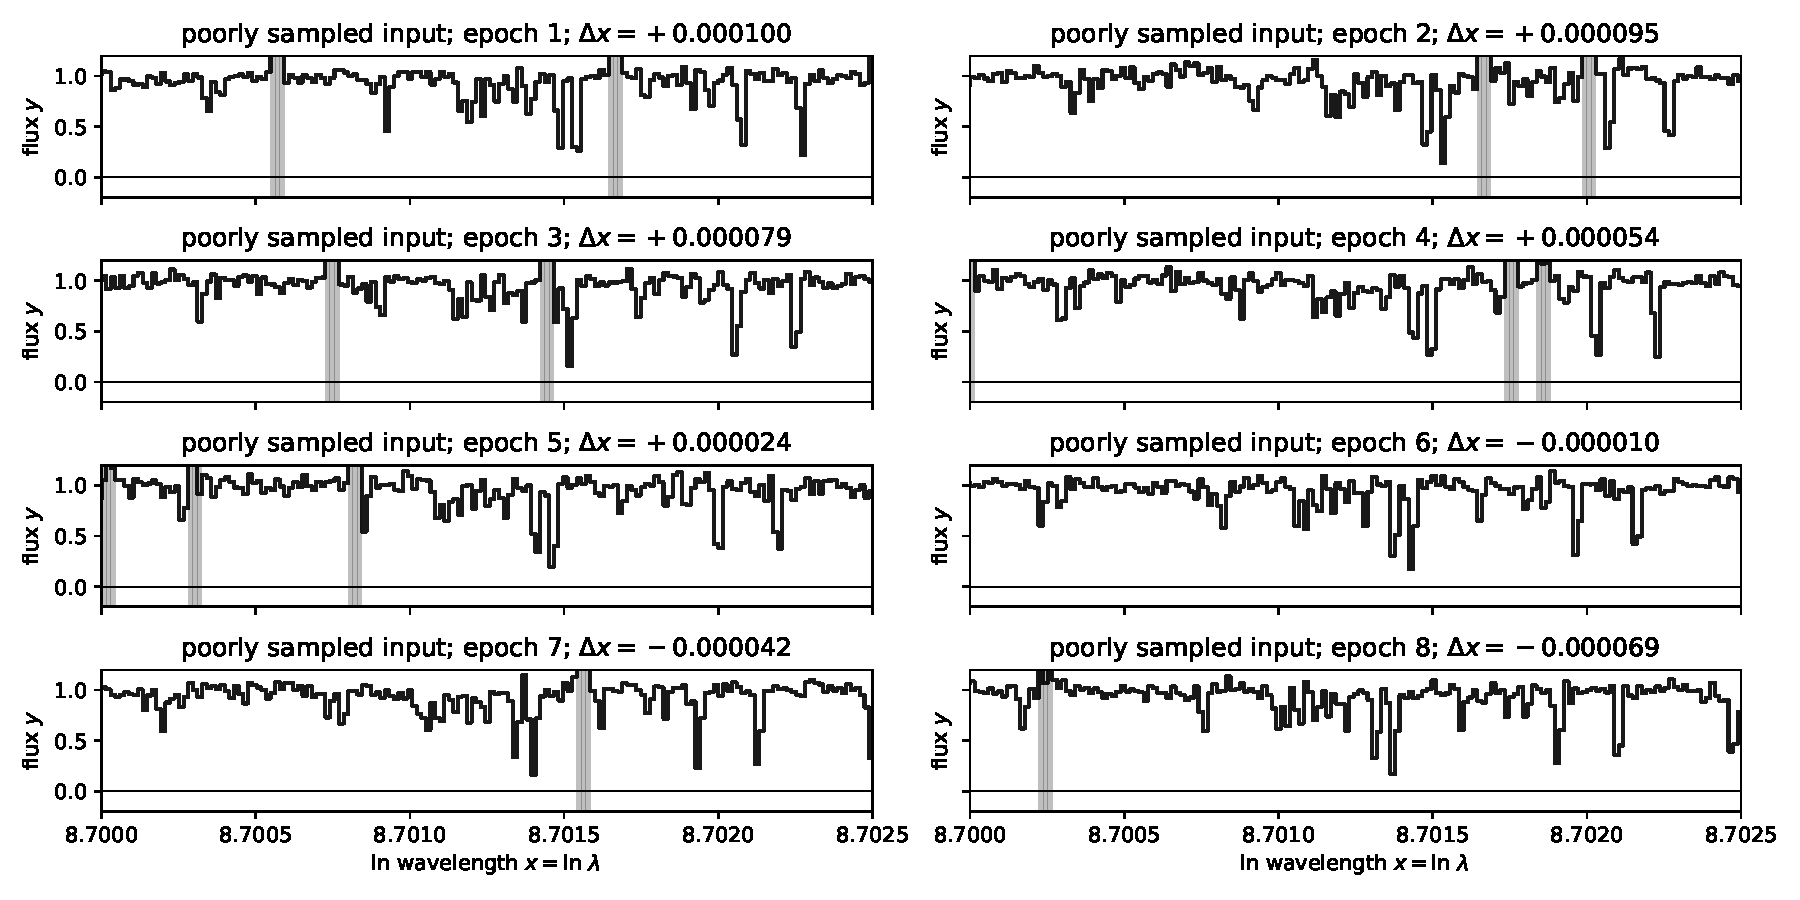
\includegraphics[width=1.3\figurewidth]{notebooks/data1.pdf}\\
    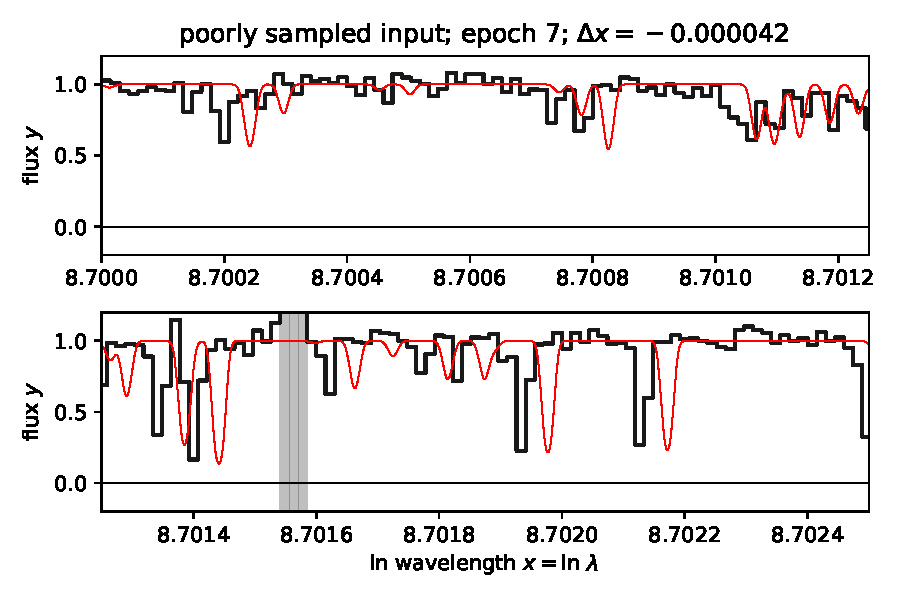
\includegraphics[width=\figurewidth]{notebooks/datazoom.pdf}
    \end{center}
    \caption{The top 8 panels show the $N=8$ epochs of the poorly sampled input data, with $N=8$, $M=171$, and signal-to-noise per pixel of 18 in the continuum. The bad pixels are indicated with grey bars. The bottom 2 panels show a zoom in on one of the epochs, along with the true spectrum used to generate the data. The true spectrum is shown at zero Doppler shift, while each epoch spectrum is at a finite Doppler shift $\Delta x_i$ relative to the spectrograph pixel grid.\label{fig:data1}}
    \end{mdframed}
\end{figure}
\begin{figure}[t!]
    \begin{mdframed}\begin{center}
    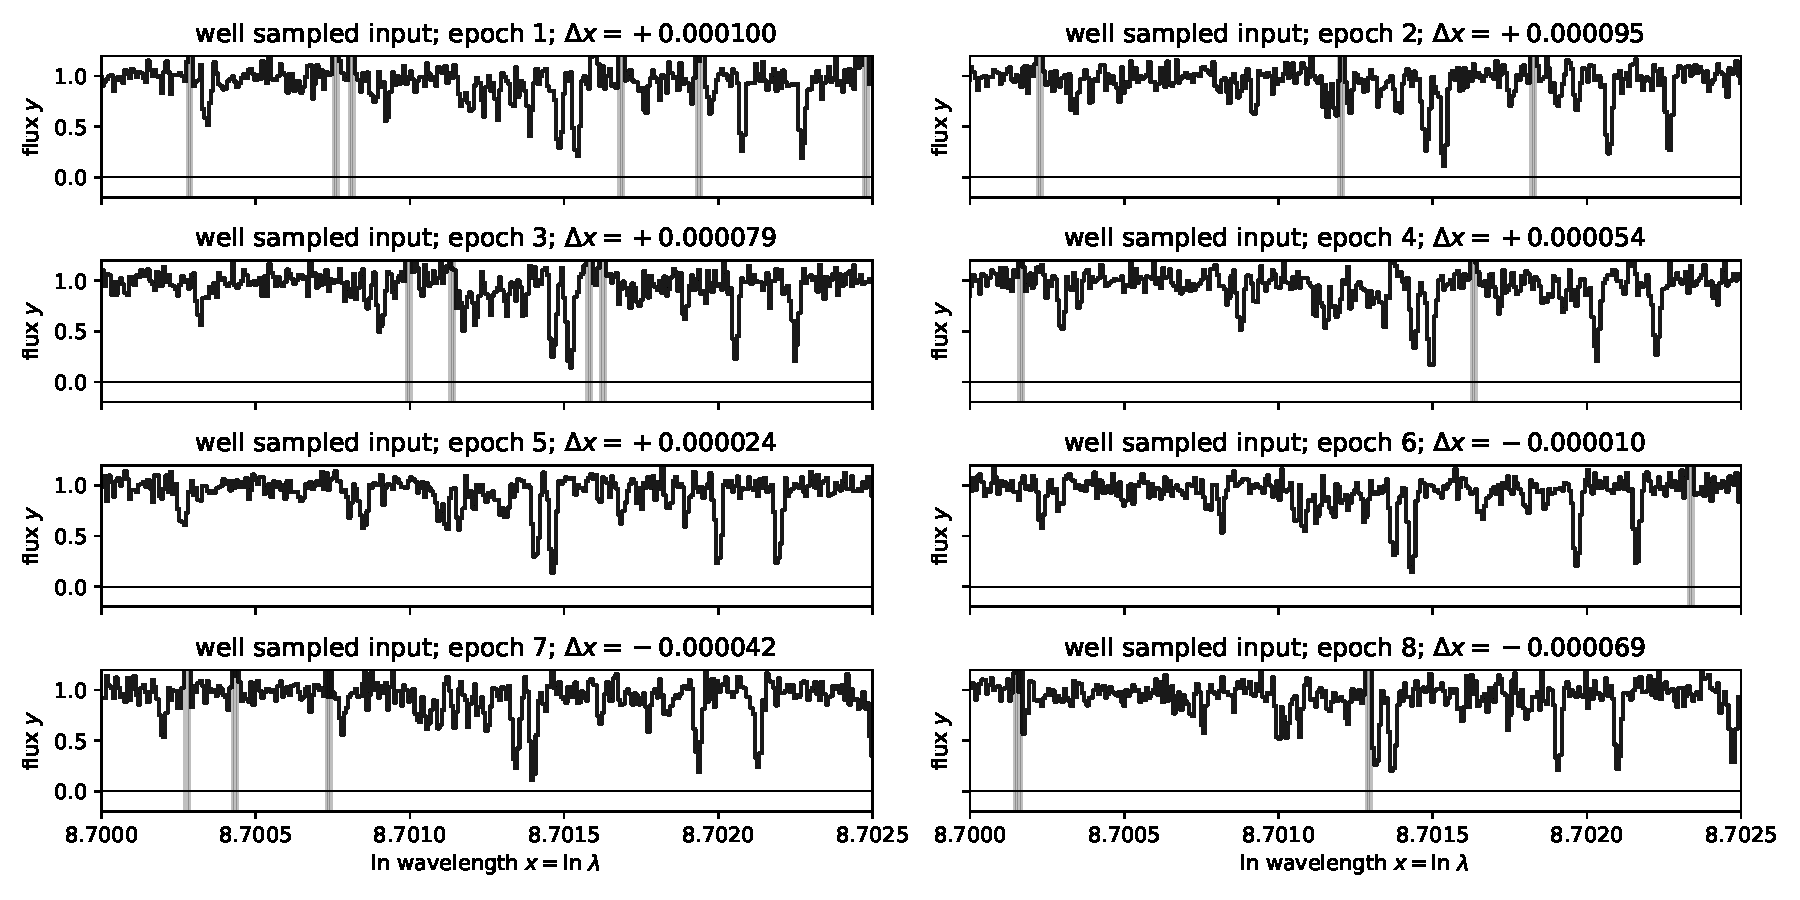
\includegraphics[width=1.3\figurewidth]{notebooks/data2.pdf}
    \end{center}
    \caption{Similar to the top panels of \figurename~\ref{fig:data1} except showing the well sampled input data with $N=8$, $M=340$, and signal-to-noise per pixel of 12 in the continuum.\label{fig:data2}}
    \end{mdframed}
\end{figure}

\paragraph{Forward Model (tm)}
As our main experiment or result, we apply the Forward Model (tm) as described above in \sectionname~\ref{sec:method} to the input data shown in \figurename~\ref{fig:data1} and \figurename~\ref{fig:data2}.
In each case, the output pixel grid $x_\star$ is chosen to be well sampled, with a pixel spacing of $1/R$ in the (natural) logarithm of wavelength.
In order to give the model maximum flexibility, the number $P$ of Fourier modes in the spectral model is set to be equal to the number of pixels $M_\star$ in the pixel representation.
The log-wavelength scale $L$ of the Fourier basis was set to the pixel spacing times the number of pixels.
We didn't employ any data weighting; we treated every epoch as identical in terms of inverse variance.

\begin{figure}[t!]
    \begin{mdframed}\begin{center}
    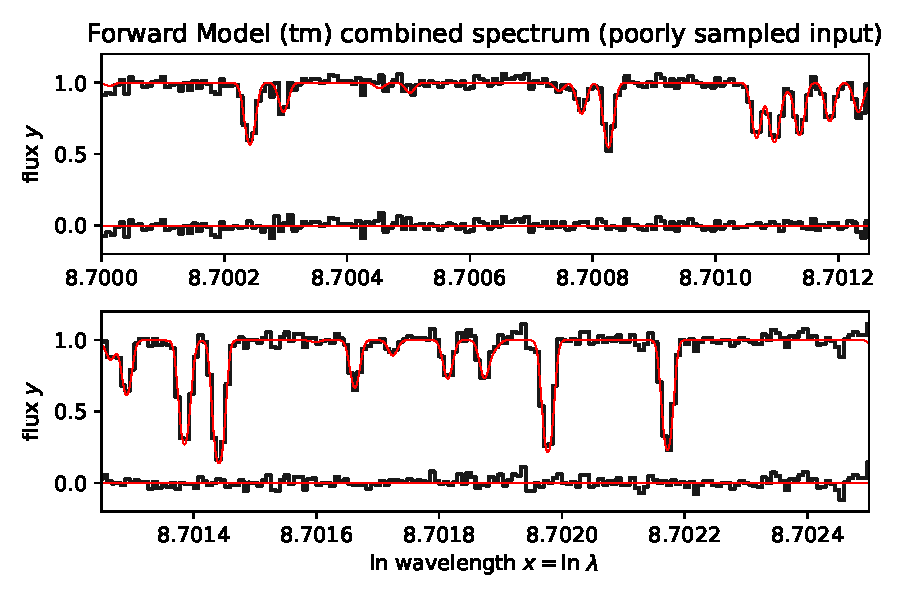
\includegraphics[width=\figurewidth]{notebooks/forward1.pdf}\\
    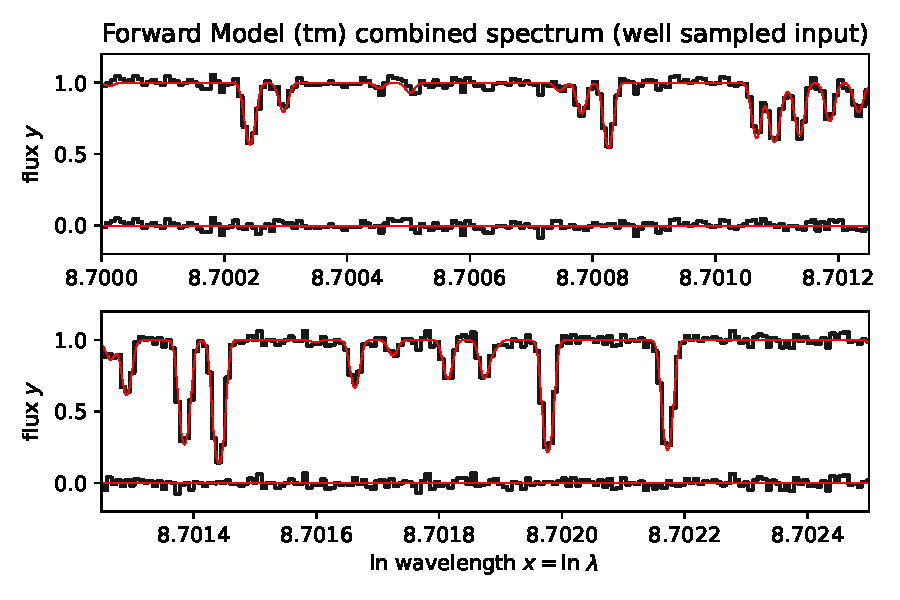
\includegraphics[width=\figurewidth]{notebooks/forward2.pdf}
    \end{center}
    \caption{The top two panels show the result of running the Forward Model (tm) on the poorly sampled input data, plus the residual away from the truth. The bottom two panels show the same but for the well sampled input data. In each panel, the red line shows the true model used to generate the data.\label{fig:forward}}
    \end{mdframed}
\end{figure}
The combined spectrum resulting from the Forward Model (tm) described in \sectionname~\ref{sec:method} is shown in \figurename~\ref{fig:forward}.
It is compared to the true spectral expectation model that was used to generate the data.
Also shown in \figurename~\ref{fig:forward} is the residuals, Forward Model (tm) minus truth.
The residuals look stationary, approximately Gaussian, and uncorrelated (more on this below).

\paragraph{Standard Practice (tm)}
In standard practice, the individual spectra $y_i$ are interpolated to rest-frame spectra $y'_i$ using an interpolator.
In detail, the data are shifted and also resampled onto the output pixel grid $x_\star$.
The interpolator is a choice; cubic spline, Lanczos, and sinc interpolations are common, since they have good properties with respect to the spectrograph band limit.
Here we choose a cubic spline for convenience, but there are many other choices, including linear, sinc, and Lanczos interpolators, among many others.

The interpolated spectra $y'_i$ are, by construction, all on the same rest-frame wavelength grid $x_\star$ so they can be averaged, with a straight average, a median, an inverse-variance-weighted mean, or any more sophisticated algorithm.
Here we choose an inverse-variance-weighted mean (HOGG: NO WE DON'T), but zeroing out the inverse variance at the locations of the bad pixels.

This censorship of the bad pixels requires some attention:
Naive interpolation of an integer (binary actually) bad-pixel mask $b_i$ will not deliver an integer mask $b'_i$.
The conservative move (which we adopt) is to naively interpolate $b_i$ (also by the cubic spline) and then zero out any pixels that are significantly below unity.
In general this substantially grows the binary mask, and reduces the amount of data available for combination.
The non-conservative approach is just as bad: if we restrict the number (or fraction) of pixels in the combined spectrum to equal those in the individual epochs, we risk un-masking genuinely bad pixels while growing the binary mask elsewhere!

\begin{figure}[t!]
    \begin{mdframed}\begin{center}
    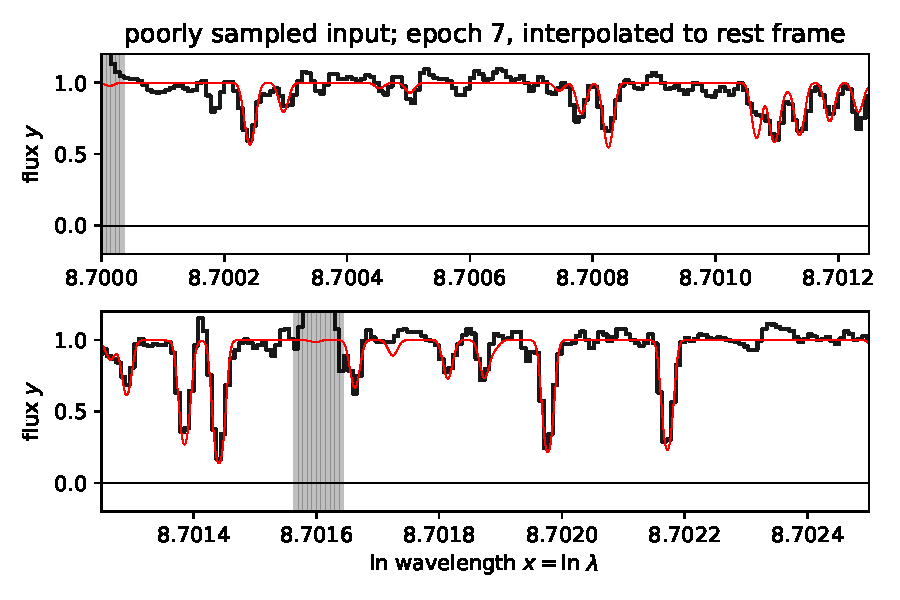
\includegraphics[width=\figurewidth]{notebooks/datazoom_interpolated.pdf}
    \end{center}
    \caption{As part of Standard Practice (tm), it is necessary to interpolate the individual epoch spectra before averaging them. This shows one epoch of the poorly sampled data, interpolated to the output $x_\star$ pixel grid in the rest frame. The interpolated spectrum is compared to the true spectral expectation employed to generate it. Note the ringing induced by the interpolation. Also shown is the censored data, near an interpolated bad pixel and at the edge of the domain. Compare to the bottom panels of \figurename~\ref{fig:data1}.\label{fig:interpolated}}
    \end{mdframed}
\end{figure}
An example of a poorly-sampled spectrum interpolated to the rest frame is shown in \figurename~\ref{fig:interpolated}.
The interpolation introduces substantial ringing artifacts in the spectrum (compare to \figurename~\ref{fig:data1}).
It also grows the bad-pixel mask around the bad pixel.

\begin{figure}[t!]
    \begin{mdframed}\begin{center}
    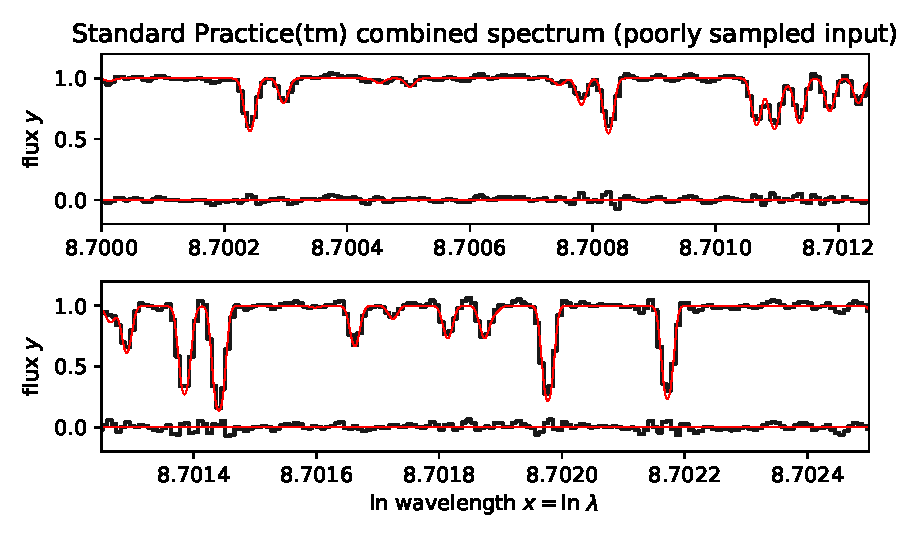
\includegraphics[width=\figurewidth]{notebooks/standard1.pdf}\\
    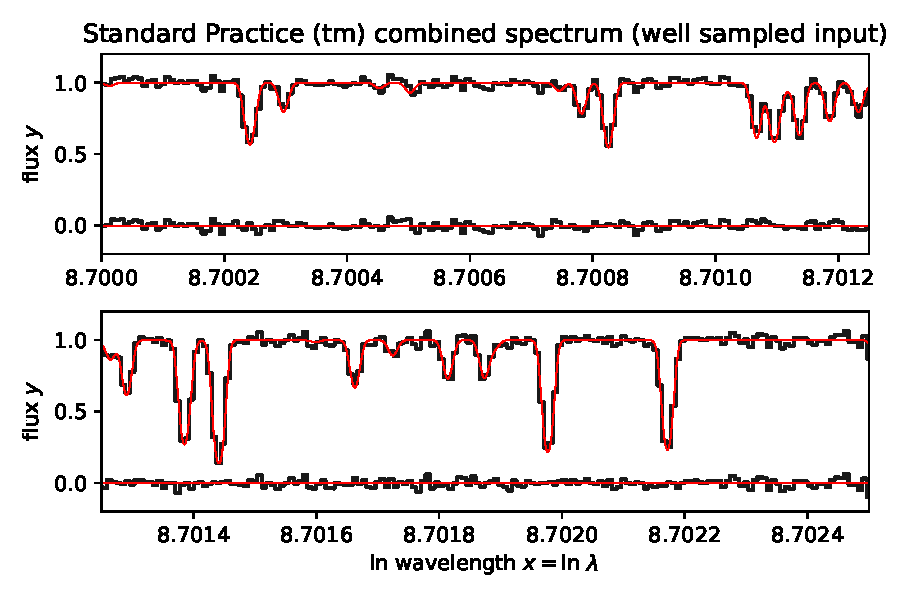
\includegraphics[width=\figurewidth]{notebooks/standard2.pdf}
    \end{center}
    \caption{Same as \figurename~\ref{fig:forward} but for the output of Standard Practice (tm). Note that in the poorly sampled case, the residuals appear to be spatially correlated, and the residuals appear to be larger near strong spectral features; more about these issues in the text and in \figurename~\ref{fig:noise}.\label{fig:standard}}
    \end{mdframed}
\end{figure}
We show the final result of Standard Practice (tm)---interpolating the input data and then averaging the interpolations---for the two data sets, in \figurename~\ref{fig:standard}.
We also show the comparison with the true spectral expectation model that was employed to make the fake data.
The residuals look correlated (there is some ringing which mimics weak spectral features), and the residuals are larger near strong spectral features, especially in the case of the poorly sampled input data.

\paragraph{Noise and noise covariances}

We repeated the above experiments to empirically measure the noise covariances, and to estimate how correlated neighboring pixels are in the output spectrum. For the poorly sampled case and the well sampled case, we generated 64 multi-epoch data sets and computed the mean spectrum using the Forward Model (tm) and Standard Practice (tm). We then computed the empirical covariance in the output spectrum minus the true spectrum, which are shown in \figurename~\ref{fig:noise}.
In each case, Standard Practice (tm) has a lower noise variance at zero lag, but shows spatially correlated noise over many pixels.
The Forward Model (tm), in contrast, shows no pixel-to-pixel noise covariances, even when the input data are ill sampled.
\begin{figure}[t!]
    \begin{mdframed}\begin{center}
    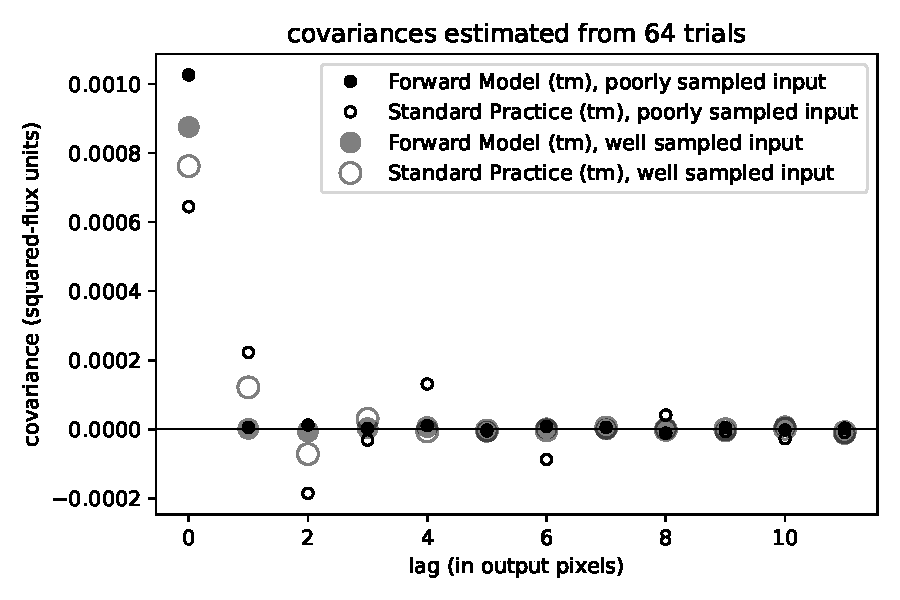
\includegraphics[width=\figurewidth]{notebooks/noise.pdf}
    \end{center}
    \caption{The empirical noise variance in the output (combined) spectra, and pixel-to-pixel covariances, as a function of pixel lag (pixel offset). The variances were estimated by performing the experiments repeated 64 times, with the same spectral expectations and sampling but unique noise draws. The Forward Model (tm) has slightly larger variance per pixel at zero lag, but vanishing pixel-to-pixel correlations. In contrast, the Standard Practice (tm) leads to correlated pixel values, with correlations extending out to many pixels.\label{fig:noise}}
    \end{mdframed}
\end{figure}

HOGG: Note that if we choose $P<M$ we start to see noise correlations in the Forward Model (tm) too.
That's one of a few reasons we like $P=M$.

\section{Discussion}\label{sec:discussion}

Give some summary of the above.
% ARC: Did you want to add summary of the above, or is this comment stale and the summary is now below?

In the Introduction, we were agnostic about whether we were talking about imaging or spectroscopic data.
In the end, our examples are spectroscopic.
What differences are there between these cases?
The main difference is that there are many more ``shift'' parameters for imaging than spectroscopy:
Two spectra (according to our assumptions) differ only (or primarily) in terms of a one-dimensional Doppler shift with respect to pixels that are located in one dimension (the wavelength direction).
Imaging epochs, on the other hand, can differ in terms of two shifts and a rotation, or (equivalently) three Euler angles.
And, since every pixel has its own two-dimensional position, the problem of locating pixels in an image is generally harder than the problem of locating pixels in an extracted spectrum.
That is, the imaging case is generally more difficult.
But it is not different, conceptually, from what is presented above.

Everything presented above depends on a set of strong assumptions, listed in \sectionname~\ref{sec:assumptions}.
Perhaps the strongest assumption is that the spectrum or image is not a function of time.
That is, each epoch spectrum or image is a sampling of the same underlying, true signal.
This assumption can be wrong for a myriad of reasons:
The source can vary, the instrument can vary, there can be variable foregrounds or backgrounds, and there can be mistakes or variations in calibration or data processing.
All of these things happen in real data sets, but the Forward Model (tm) is no more impacted by this than what is done in Standard Practice (tm)!

There are (at least) three attitudes for an investigator to take in the face of variations in the data, from epoch to epoch or exposure to exposure:
The first is that the procedures we design are designed to deliver the exposure (or signal-to-noise-squared) weighted mean of the observed epochs.
That is, the fact that the data are varying does not mean that the methodology needs to be modified; without modification, the procedures given above---both the Forward Model (tm) and the Standard Practice (tm)---will produce something like the mean spectrum.

The second attitude to take---and the necessary attitude for many projects---is that the variations must be accounted for, by complexifying the forward model.
For example, if there is a varying line-spread function between epochs (as there is for the \textsl{APOGEE} spectrograph, because the LSF is a function of the slit position of the optical fiber), then in addition to a shift at each epoch there is also an LSF adjustment at each epoch.
The LSF adjustment is then applied to the spectral model before it is compared to each epoch of data, just as the shift is applied in the current methodological scope.
Similar model adustments can account for intrinsic spectral variations, additive or multiplicative nuisance signals in the data (like backgrounds or telluric absorptions), and mistakes in data pre-processing (like continuum modeling errors).

One side note about epoch-to-epoch variations in instrument or data-processing parameters:
It is usually a good idea to model not the full instrument or data properties (as does \citealt{sp}) if that can be avoided, but rather just the \emph{differences} in instrument or data properties from one epoch to the next, taking those differences away from some fiducial data or instrument state.
In the case of the LSF, for example, that obviates the need to model the infinite-resolution spectrum; the spectrum only needs to be modeled at fiducial resolution and convolved to other resolutions with difference kernels.

Although \emph{conceptually} changes to account for data variability aren't that big, \emph{in practice} they can be very hard to implement.
For one, the method we have presented assumes that we \emph{know} the individual epoch shifts \textsl{a priori}, and all new epoch-to-epoch adjustments would also depend on per-epoch housekeeping data or parameters that might, in practice, be hard to know.
That brings us to the third attitude that the investigator can take.
What's presented above can be seen as a model for the \emph{mean} of the process that generates individual-epoch spectra; that is the first term in an expansion of moments.
The next term would be the \emph{variance} of the process.
That is, a more sophisticated model could have not just $P$ parameters for the mean spectrum, but additionally $P'$ parameters for a variance model.
If the variance is low dimensional, or sparse, or compact in important ways, there should be very effective models of this form.
For example, we could imagine forward-modeling generalizations of some of sparse methods (for example, \citealt{candes}) for applications in which the variability is localized in time or space; or we could imagine generalizations of matrix factorizations (for example, \citealt{hmf}) for applications in which variability is low dimensional (the \textsl{wobble} method has some such functionality; \citealt{wobble}). % HOGG: need candes and hmf citations

All the above considerations of variability bring us to another of our strong assumptions:
We have assumed that we know the shifts $\Delta x_i$ exactly.
In practice, we rarely do, or maybe more accurately: We rarely know them as well as we could know them, in principle.
When the shifts $\Delta x_i$ are not known, or not known accurately enough, we recommend a simultaneous-fitting procedure, in which the shifts are learned at the same time as the combined spectrum is estimated or inferred.
This can be achieved through a challenging nonlinear optimization, or through an iteration of linearized optimizations, alternating improvements to the combined spectrum and improvements to the shifts.
This is, more or less, how the \textsl{wobble} system works (\citealt{wobble}).

% What about non-Gaussian noise?

We assumed that the noise was Gaussian, but this is not always true of astronomical data.
In the case of Poisson noise that is not background dominated, the variance tensor $C_i$ will be biased, and all our assumptions about additive Gaussian variance will be broken. % ARC: what else should we say about this?


Code is available at \url{https://github.com/davidwhogg/NoDataInterpolation} and is registered in the Python Package Index as \texttt{NoDataInterpolation}.

\paragraph{Software}
\texttt{numpy} \citep{numpy} ---
\texttt{matplotlib} \citep{matplotlib}.

\paragraph{Acknowledgements}
It is a pleasure to thank
Mike Blanton (NYU),
Matt Daunt (NYU),
Jon Holtzman (NMSU), 
Dustin Lang (Perimeter),
Adrian Price-Whelan (Flatiron),
and the Astronomical Data Group at the Flatiron Institute,
for valuable discussions and input.

\begin{thebibliography}{dummy}
\bibitem[Barnett et al.(2019)]{finufft}
Barnett, A. H., Magland, J. F., \& af~Klinteberg, L., 2019, SIAM J. Sci. Comput. 41(5), C479
\bibitem[Bedell et al.(2019)]{wobble} Bedell, M., Hogg, D.~W., Foreman-Mackey, D., et al.\ 2019, \aj, 158, 164. doi:10.3847/1538-3881/ab40a7
\bibitem[Bolton \& Schlegel(2010)]{sp} Bolton, A.~S. \& Schlegel, D.~J.\ 2010, \pasp, 122, 248. doi:10.1086/651008
\bibitem[Harris et al.(2020)]{numpy} Harris, C.~R., Millman, K.~J., van der Walt, S.~J., et al.\ 2020, \nat, 585, 357. doi:10.1038/s41586-020-2649-2
\bibitem[Hewett et al.(1985)]{oe} Hewett, P.~C., Irwin, M.~J., Bunclark, P., et al.\ 1985, \mnras, 213, 971. doi:10.1093/mnras/213.4.
\bibitem[Hogg et al.(2010)]{fitting} Hogg, D.~W., Bovy, J., \& Lang, D.\ 2010, arXiv:1008.4686
\bibitem[Hogg \& Villar(2021)]{fittingflexible} Hogg, D.~W. \& Villar, S.\ 2021, \pasp, 133, 093001. doi:10.1088/1538-3873/ac20ac
\bibitem[Hunter(2007)]{matplotlib} Hunter, J.~D.\ 2007, Computing in Science and Engineering, 9, 90. doi:10.1109/MCSE.2007.55
\bibitem[Ivezi{\'c} et al.(2019)]{lsst} Ivezi{\'c}, {\v{Z}}., Kahn, S.~M., Tyson, J.~A., et al.\ 2019, \apj, 873, 111. doi:10.3847/1538-4357/ab042c
\bibitem[Majewski et al.(2017)]{apogee} Majewski, S.~R., Schiavon, R.~P., Frinchaboy, P.~M., et al.\ 2017, \aj, 154, 94. doi:10.3847/1538-3881/aa784d
\bibitem[Williams et al.(1996)]{hdf} Williams, R.~E., Blacker, B., Dickinson, M., et al.\ 1996, \aj, 112, 1335. doi:10.1086/118105
\bibitem[Wilson et al.(2019)]{apogeehardware} Wilson, J.C., Hearty, F.R., Skrutskie, M.F., Majewski, S.R., Holtzman, J.A., Eisenstein, D., et al.\ 2019, \pasp, 131, 055001. doi:10.1088/1538-3873/ab0075.
\bibitem[Wolf et al.(2003)]{combo17} Wolf, C., Meisenheimer, K., Rix, H.-W., et al.\ 2003, \aap, 401, 73. doi:10.1051/0004-6361:20021513
\bibitem[Zechmeister et al.(2014)]{froe} Zechmeister, M., Anglada-Escud{\'e}, G., \& Reiners, A.\ 2014, \aap, 561, A59. doi:10.1051/0004-6361/201322746
\end{thebibliography}

\end{document}
